\documentclass{article}
\usepackage[utf8]{inputenc}
\usepackage{amsmath}
\usepackage{amsfonts}
\usepackage{graphicx}

\title{Written Assignment Unit 7\\
Math 1201- College Algebra.
}
\author{Instructor - Casmir Onyeneke}
\date{October 2021}
\begin{document}

\maketitle


\section*{PART 1}
\title\textbf{QUESTION}\\
Find the length of an arc in a circle of radius 10 centimeters subtended by the central angle of ${50^{\circ}}$. Show your work.\\
\\\title\textbf{SOLUTION}\\
The length of an arc, ${l}$ is given by the formula (Abramson, 2017).
$${l = \frac{\theta}{360}\times 2\pi r}$$
where:\\ 
$\theta$ is the angle subtended by the arc, and \\
r is the radius of the arc.
Now, from the question $\theta = 50^{\circ}$, and r = 10cm
Substituting into the formula,  
$${l = \frac{50}{360}\times 2\times\pi\times10 }$$
$${l = \frac{5}{36}\times 20\times\pi}$$
$${l = \frac{100}{36}\times\pi}$$
$${l = 2.78 \ times 3.142}$$
$${l = 8.73476}$$
Therefore the length of the arc, ${l}$ is approximately $8.73cm$

\section*{PART 2}
\title\textbf{QUESTION}\\
Graph ${f(x) = x sin x}$ on $[-4\pi, 4\pi]$ and verbalize how the graph varies from the graphs of ${f(x) = \pm x}$\\
Graph ${f(x) =\frac{sinx}{x}}$ on the window $[-5\pi, 5\pi]$ and describe freely what the graph shows. You can use www.desmos.com/calculator to obtain the graphs.\\
\\\title\textbf{2a Solution}\\
The graph of ${f(x) = x sin x}$ on $[-4\pi, 4\pi]$ and ${f(x) = \pm x}$\\
\\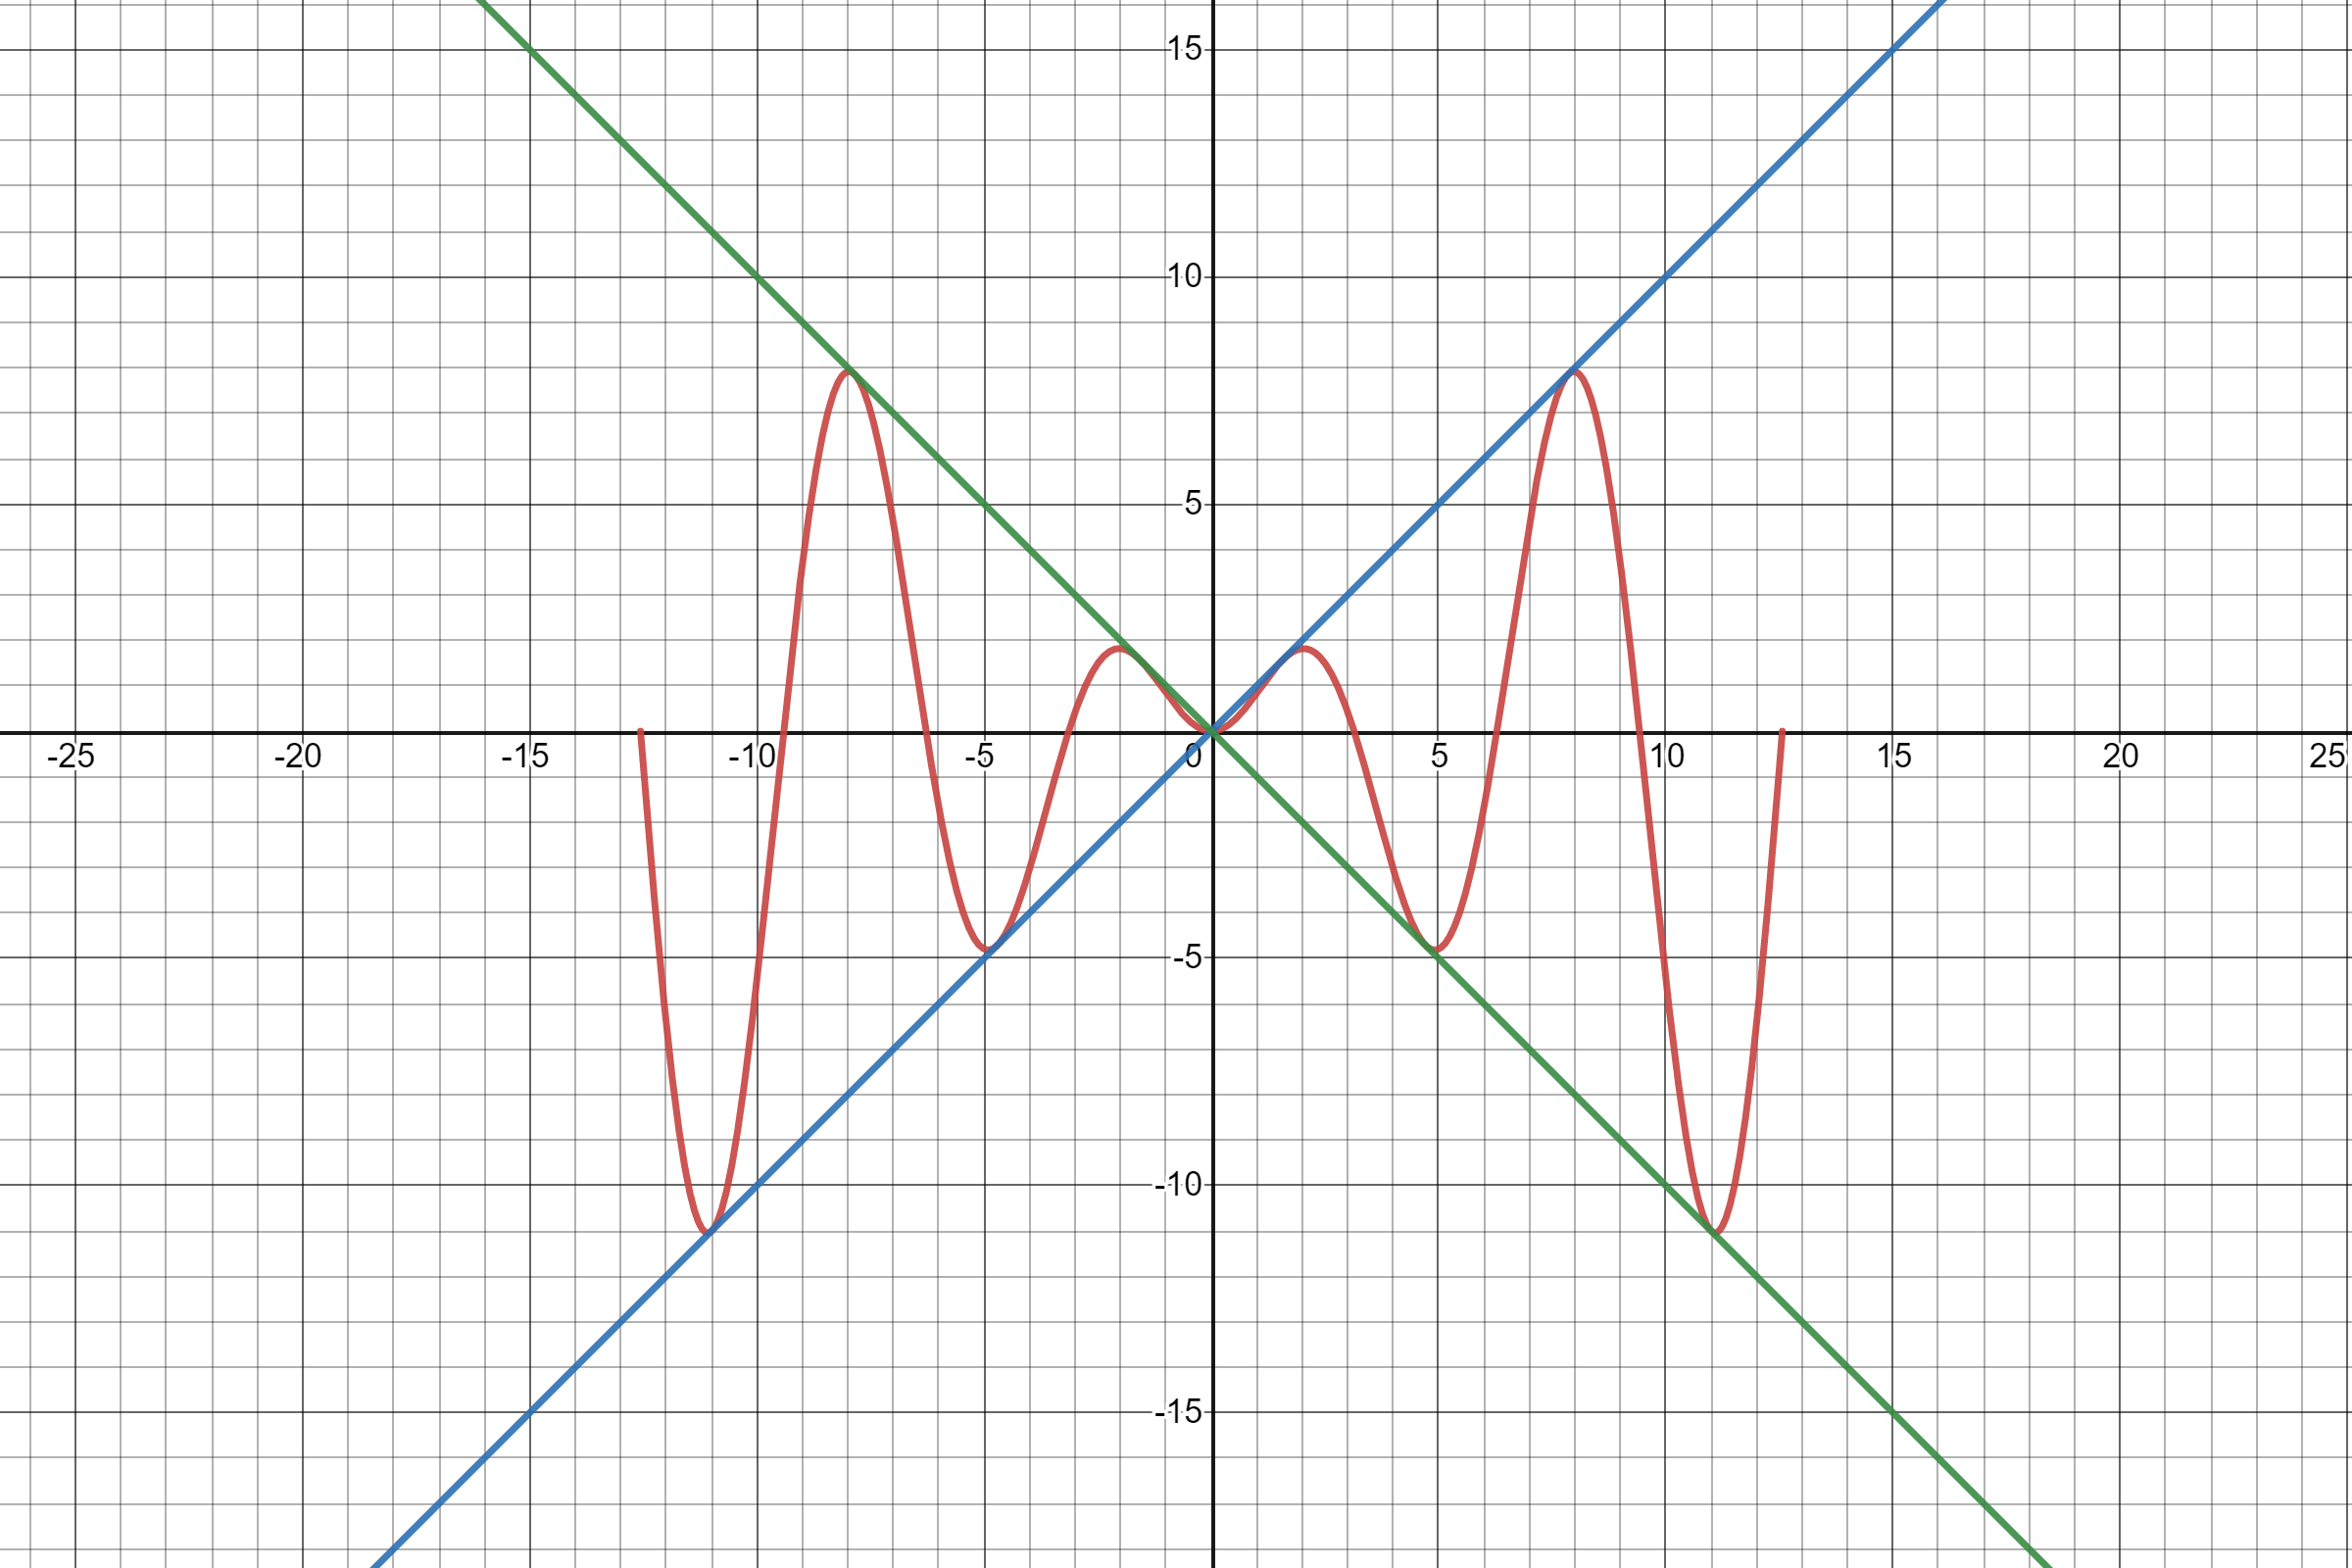
\includegraphics[scale = 0.15]{Q2a}\\
Below are my observations of about both graphs\\
\begin{enumerate}
    \item The graph of ${f(x) = x sin x}$ is non-linear and sinusoidal, while the graph of ${f(x) = \pm x}$ is linear (Abramson, 2017).
    \item The graph of ${f(x) = x sin x}$ when ${-4\pi \le x \le 0}$ is reflected when ${0 \le x \le 4\pi}$
    \item The turning points of the graph of ${f(x) = x sin x}$ lies at the points of intersection with the graph ${f(x) = \pm x}$ (Abramson, 2017).
\end{enumerate}
\title\textbf{2b Solution}\\
The graph of  ${f(x) =\frac{sinx}{x}}$ on the window $[-5\pi, 5\pi]$\\
\\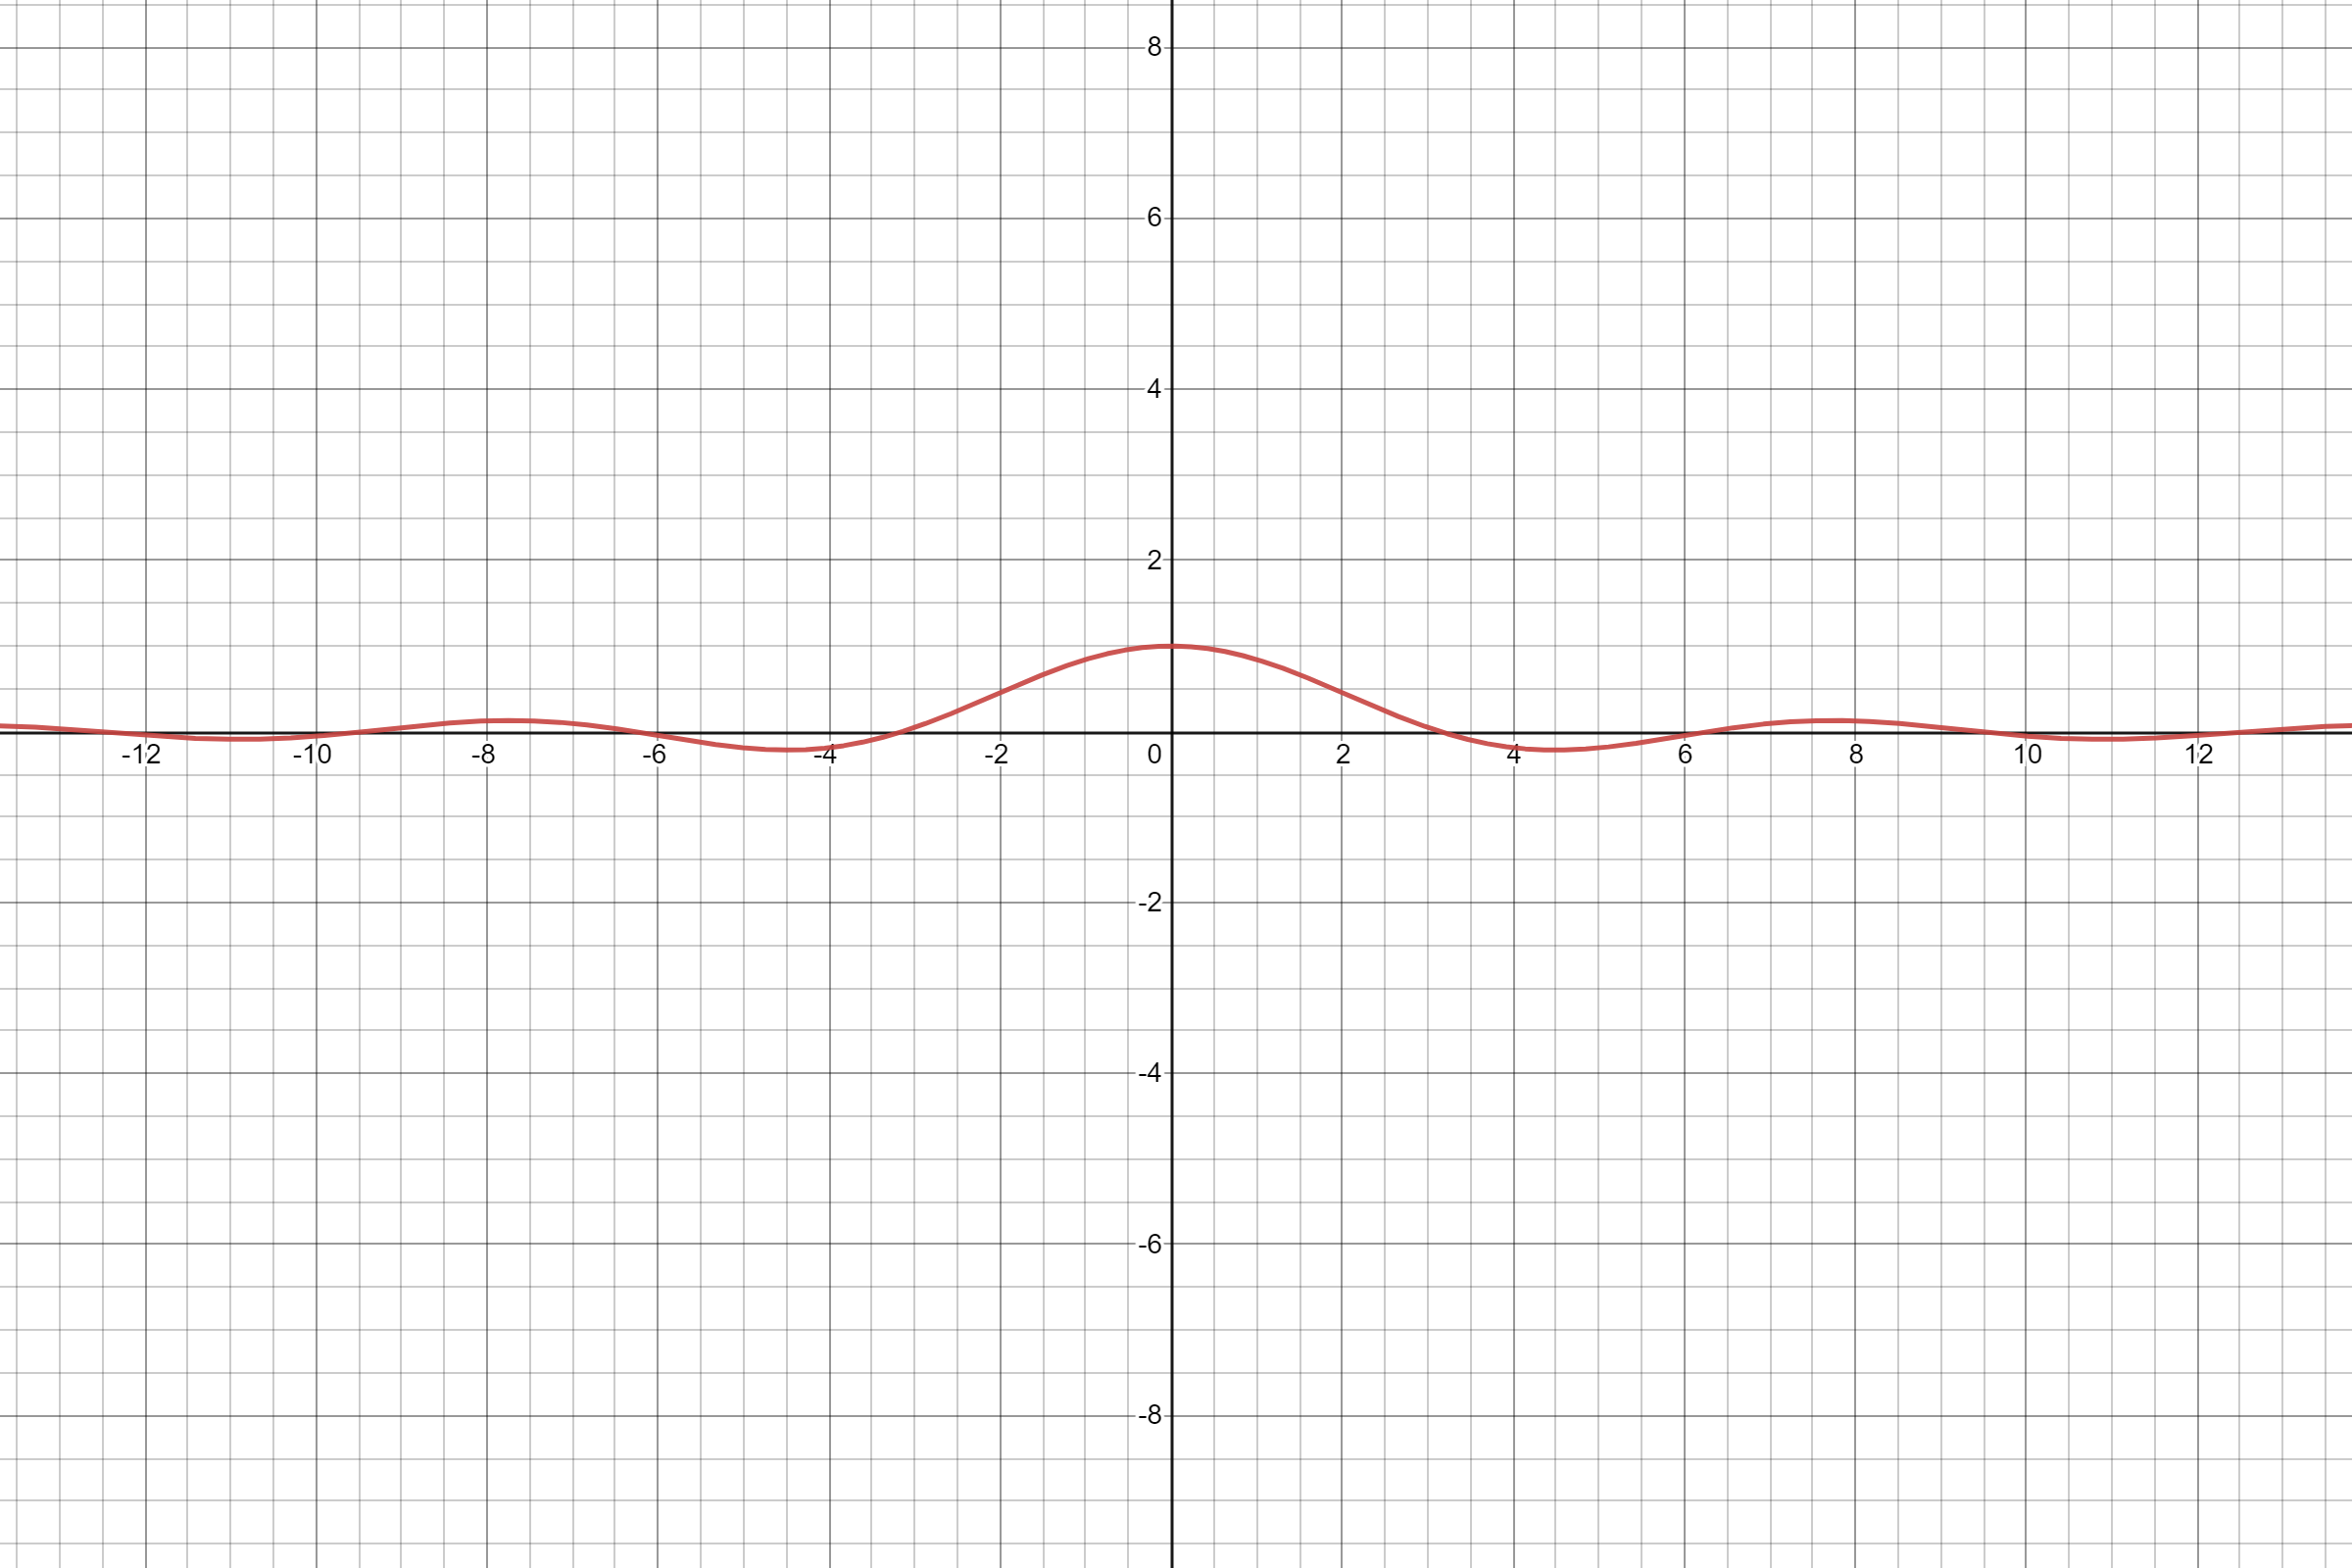
\includegraphics[scale = 0.15]{Q2b}\\
Below are my observations of the graph of ${f(x) =\frac{sinx}{x}}$\\
\begin{enumerate}
    \item The graph of ${f(x) = \frac{sinx}{x}}$ when  ${-5\pi\le x \le 0}$ is reflected when ${0 \le x \le 5pi}$ (Abramson, 2017).
    \item As the value of ${x}$ tends to ${0}$ from both ends (i.e. $-5\pi\text{ or } 5\pi$) the value of ${f(x)}$ increases.
    \item As the value of ${x}$ moves away from 0, the value of ${f(x)}$ decreases.
\end{enumerate}

\section*{PART 3}
\title\textbf{QUESTION}\\
A 23-ft ladder leans against a building so that the angle between the ground and the ladder is ${80^{\circ}}$. How high does the ladder reach up the side of the building? show the steps of your reasoning(Abramson, 2017).\\
\\\title\textbf{Solution}\\
From the question, the angle formed between the building and the ground is a right-angle, and also since the ladder is slanted in such a way that it touches both the ground and the building we can construct a right-angled triangle(Abramson, 2017).\\
To calculate how high the ladder reaches up the side of the building I would be making use of SOH from the SOH CAH TOA method of solving trigonometric problems(Abramson, 2017).\\
Now SOH is given as 
$${sin\theta = \frac{opposite}{hypotenuse}}$$
Where,\\
\begin{itemize}
    \item $\theta$ is the angle between the ladder and the ground, which is given as ${80^{\circ}}$.
    \item The Hypotenuse is the length of the ladder, which is given as $23ft$.
    \item The Opposite is how high the ladder reaches the side of the building, thus the unknown which is represented as $xft$.
\end{itemize}
Substituting these values into the SOH formula,
$${sin\theta = \frac{opposite}{hypotenuse}}$$
$${sin 80^{\circ} = \frac{x}{23}}$$
Multiply both sides by 23
$${sin 80^{\circ} \times 23 = \frac{x}{23} \times 23}$$
$${23 \times 0.9848 = x}$$
$${x = 22.65ft}$$
Therefore the height the ladder reaches on the side of the building is ${22.65ft}$.


\section*{References}
Abramson, J. (2017). \textit{Algebra and trigonometry}. OpenStax, TX: Rice University. Retrieved
from https://openstax.org/details/books/algebra-and-trigonometry
\end{document}